	Questionnaires are defined as instruments to collect data. Typically, they are composed of questions and instructions to guide the flow through an interview. With the introduction of \gls{cai} systems, these have been extended with additional features. There are two studies that explore the different constructs required to specify questionnaires. The first approach, proposed by Katz \cite{proc:katz97}, describes the different tasks involved in creating specifications for questionnaires whereas the second proposal, introduced by Bethlehem \cite{proc:bethlehem00}, uses an object-oriented paradigm to better understand all the features of an electronic questionnaire.

	In order to describe all the different constructs that may be used to construct questionnaires, we present in Figure \ref{fig:background:survey} a questionnaire intended to unify the efforts from Katz and Bethlehem. The most common types of questions are \emph{single-response}, \emph{multiple-response} and \emph{open-ended} (e.g. Q1, Q3 and Q5 respectively) whilst \emph{grid} (e.g. Q4) unlike the common types is naturally more cognitively demanding on the interviewee since more than one question in the form of rows is asked \cite{web:bock13}.

	Usually questionnaires are divided into \emph{sections} where \emph{intro} statements (e.g. INF1, INF2, END) become helpful to establish the context and introduction to a part of the questionnaire. For instance, in this example, there are two sections used to organise the set of questions, the outer section for INF1, Q1, Q2, Q3, Q4, Q5, INF2 and END and an inner for Q6a which can be asked multiple times. 

	The \emph{instructions}, in bold font, are normally included to manage questionnaire routing according to interviewee responses. There are three such routing constructs describing the flow through the questionnaire in our example:

	\begin{itemize}
		\item \emph{skip} feature allows the interviewee to skip over questions to move on to another question. This can be an \emph{unconditional} skip, as in the case of skips associated with responses in Q1 or Q2; or a \emph{conditional} skip, presented in Q5.
		\item \emph{filter} constructs are based on a logical expression involving the responses to one or more questions. They are described as if-then-else statements, for instance the instructions attached over Q5 or INF2 and also known as complex branching.
		\item \emph{loop} feature permits repeated execution of a questionnaire sub-part. For example, the instruction over Q6a defines a loop that iterates a maximum of four iterations over the selected responses from Q2 and Q3.
	\end{itemize}

	In addition to the constructs listed above, there are further features which are less frequent but nevertheless are also featured in questionnaire design.

	\begin{itemize}
		\item \emph{Piping} which allows retrieving responses from one or more previous questions as part of the text for another (e.g. question text for Q6a) or generating a set of responses based on an expression (e.g. Q3 responses are generated automatically according to those responses not mentioned in Q2).
		\item \emph{Randomising} or \emph{Rotating} features which reduce bias evasive responses by altering the data order presented to the user \cite{art:warner65} (e.g. the random presentation of the question Q6a).
		\item \emph{Computation} constitutes the execution of an arithmetical expression and its assignment over a reference variable. Typically it is used to communicate responses among sections. For example, after Q6a a stateful variable is needed to capture all the affirmative responses for Q6a. This global variable is used later as part of the filter condition associated with INF2.
		\item \emph{Check} allows the functionality to establish whether or not a logical expression is being satisfied and thereafter to notify the respondent about any inconsistencies. These constructs are helpful for a post-validation of constraints. For instance, a case in which a respondent answered that she is a non-smoker and later responds to a question as spending money on buying cigarettes. In this example, this construct could warn the respondent about such as inconsistency.
	\end{itemize}

	\begin{figure}[H]
	\centering
	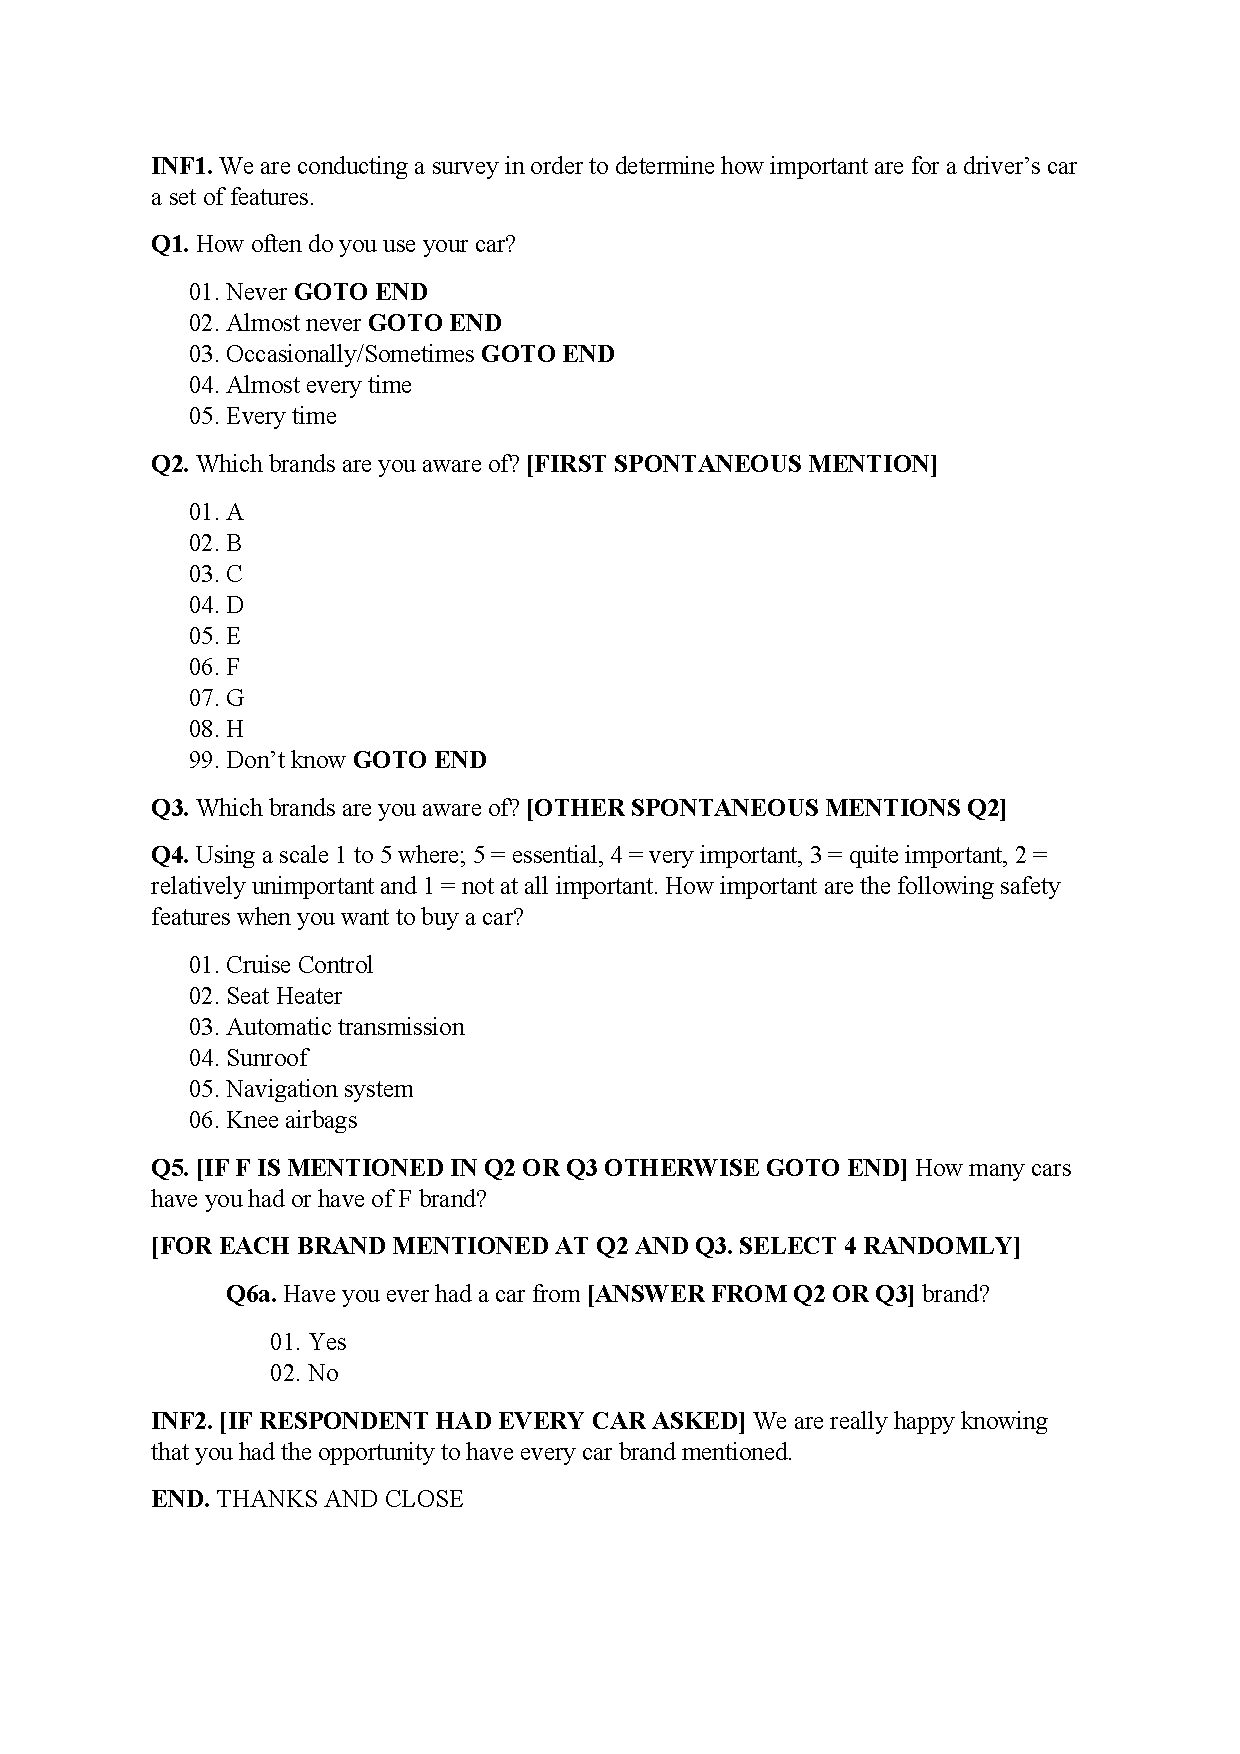
\includegraphics[max size={\textwidth}{\textheight}]{background/img/survey.pdf}
	\caption{Fully functional paper questionnaire instance}
	\label{fig:background:survey}
	\end{figure}

	
